\setauthor{Moritz Eder}

Personen, die oft gestresst vom Alltag sind, sollen durch Relaxoon wieder runterkommen können
und sich entspannen können, damit man sich wieder mit mehr Energie und einem klaren Kopf den
nächsten Aufgaben stellen kann.

Das Projekt soll zeigen, dass unter Verwendung des Open-Source headless CMS 'Strapi' und des mobilen
React-Native Frontends einfach eine App zur Wiedergabe von Mediendateien für verschiedene mobile Betriebssysteme
und zur Stressbewältigung erstellt werden kann. 


\begin{figure}[H]
    \begin{minipage}{0.5\textwidth}
        \centering
        
\includegraphics[height=0.2\textwidth]{./pics/strapi-logo.png}
        \caption{Logo Strapi}
    \end{minipage}
    \begin{minipage}{0.5\textwidth}
        \centering
        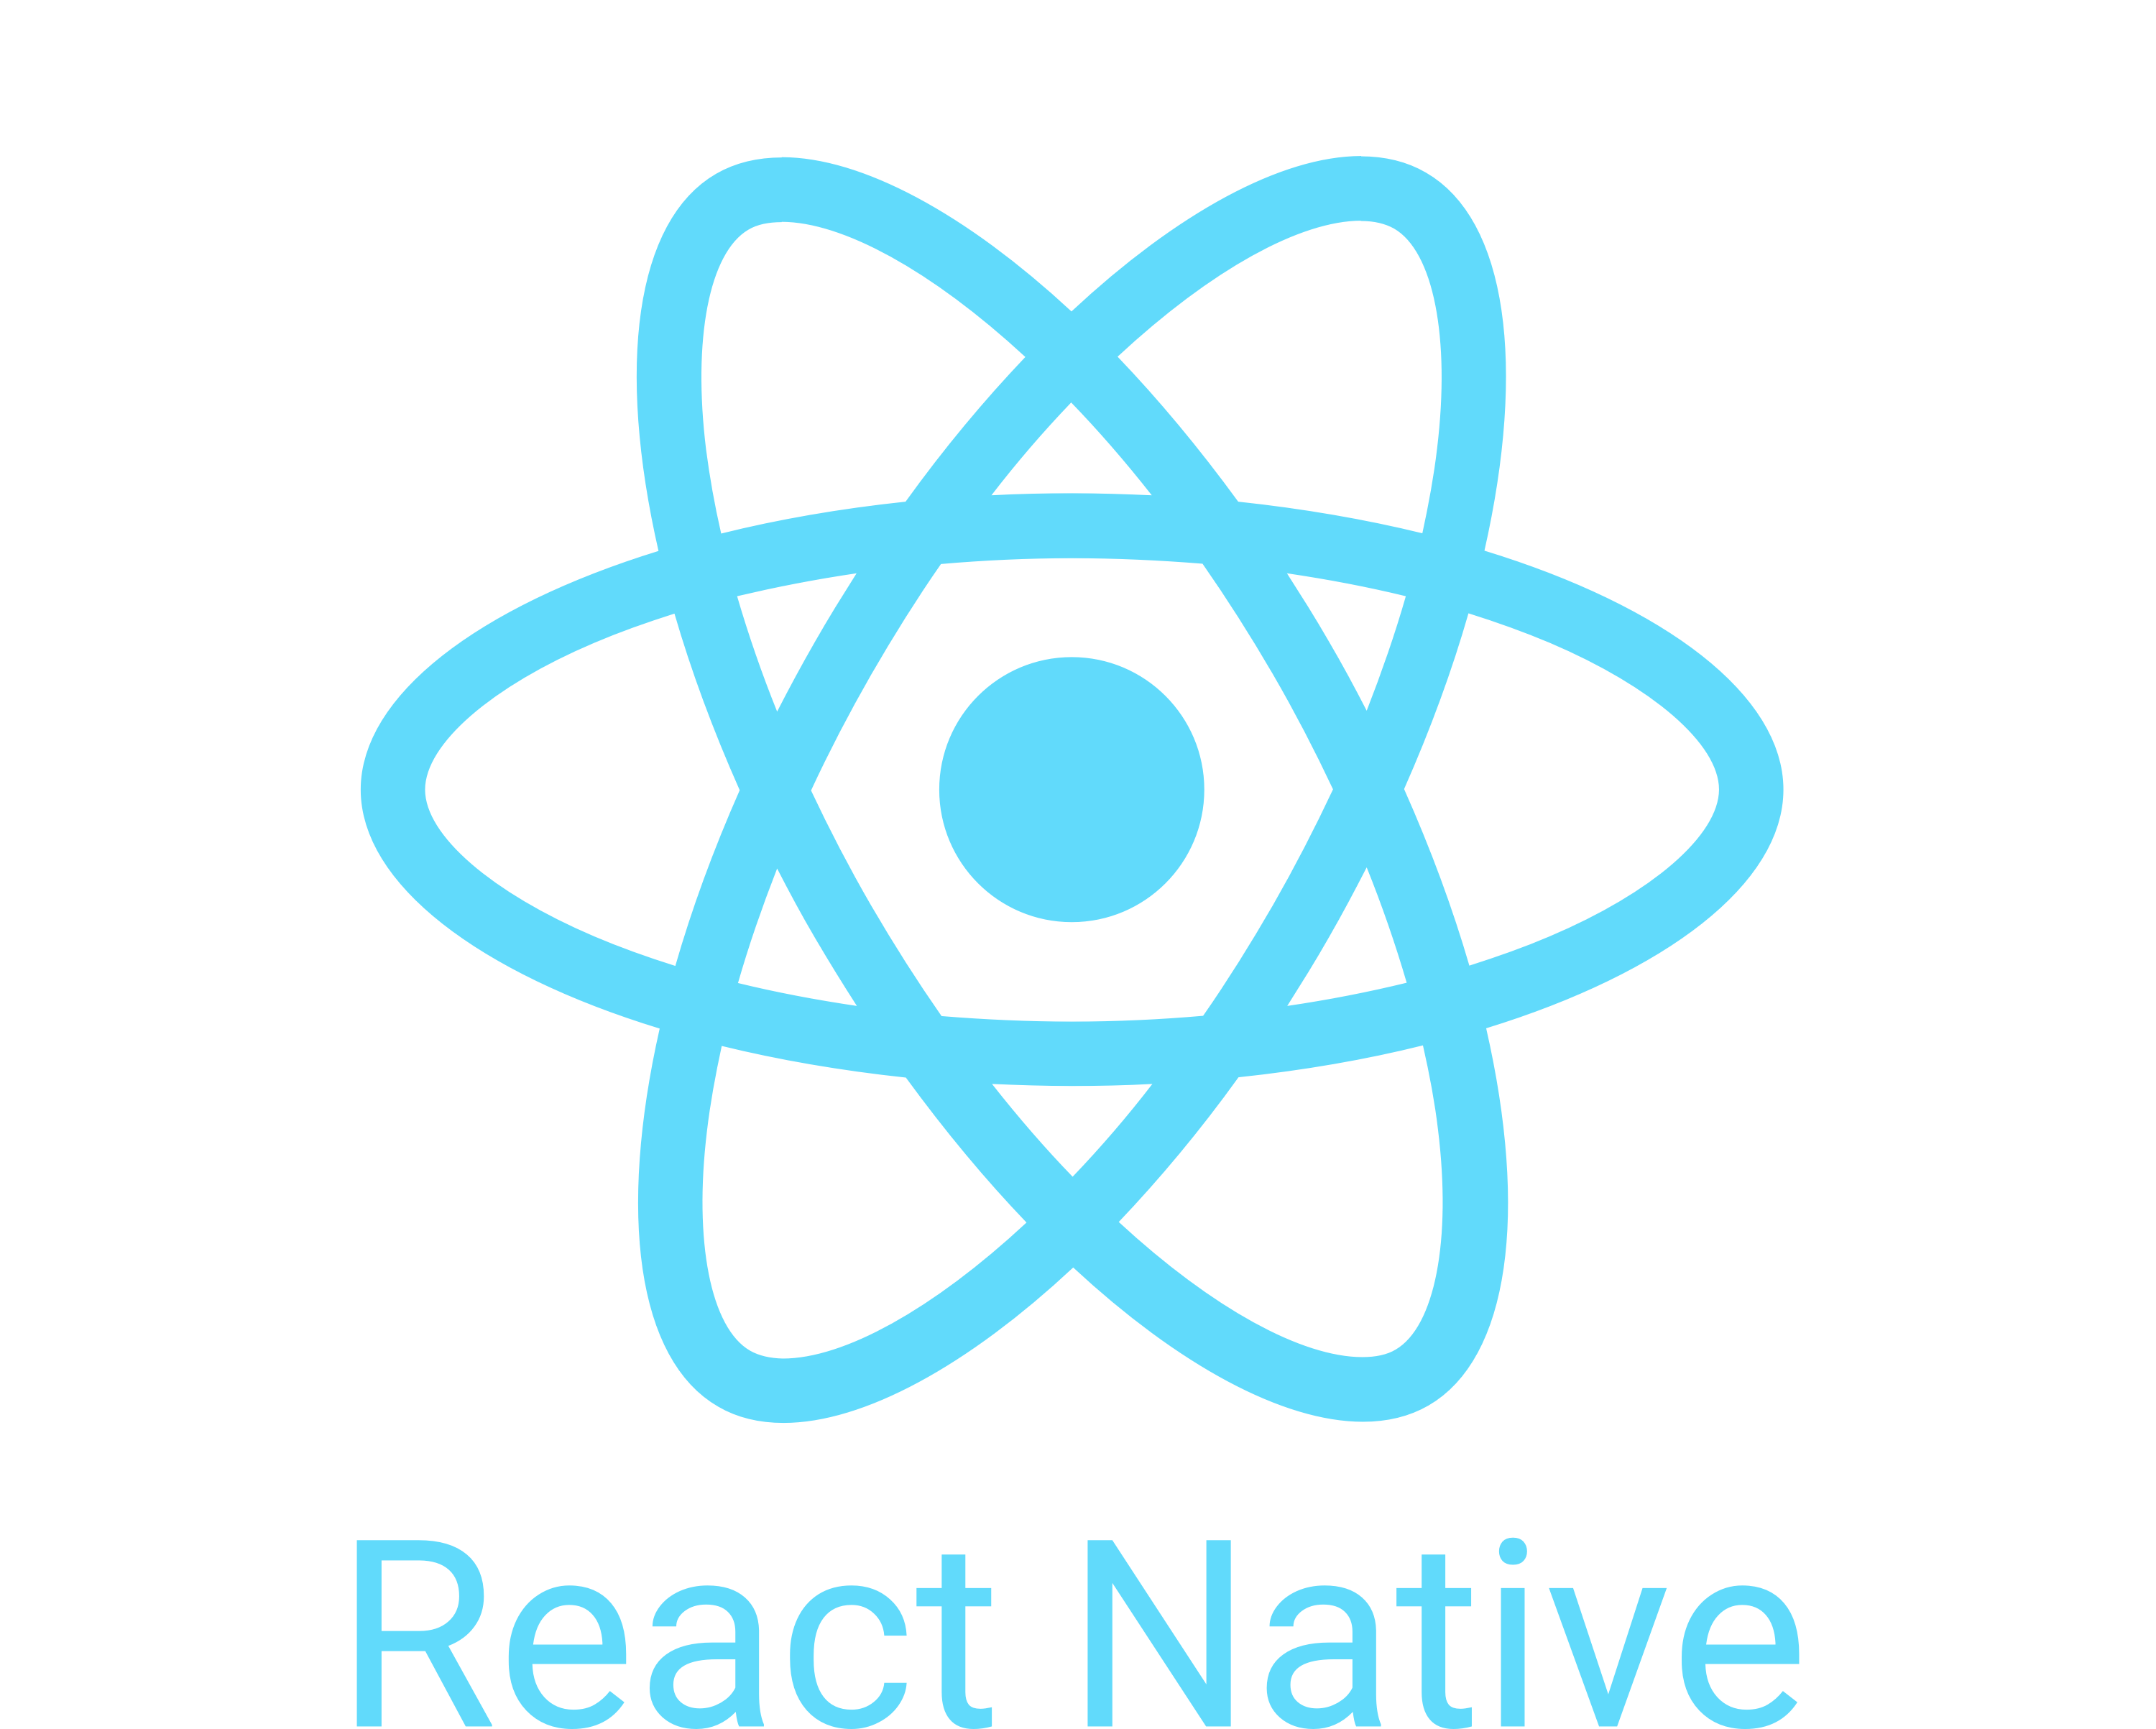
\includegraphics[height=0.6\textwidth]{./pics/react-native-logo.png}
        \caption{Logo React Native}
    \end{minipage}
\end{figure}

Wichtig dabei ist: 

\begin{itemize}
    \item Die Feinabstimmung der Qualität der Inhalte
    \item Die optimale Bereitstellung der sorgfältig ausgewählten Inhalte
    \item Ein ansprechendes und benutzerfreundliches Design für den passenden Look and Feel der App.
\end{itemize}

User:innen müssen sich in der App nicht um die eigene Erstellung von Entspannungsmedien wie Texten oder Videos
kümmern, weil diese Medien bereitgestellt werden, welche im Backend eingepflegt sind. Weiters sollen Medien
individuell favorisierbar und mehreren Kategorien zugeteilt sein, die per Suchleiste in der App einfach zu
finden sind.

Das Minimum Viable Product (MVP) von Relaxoon soll realisiert werden, damit möglichst früh Feedback von Nutzer:innen
eingeholt werden kann, welches für die Weiterentwicklung und für die Verbesserung einer App essenziell ist.

Dies bestätigt der deutsche Content-Autor Philipp Steubel, der sich im amerikanischen Softwareunternehmen auf 
die Bereiche Marketing und 
Projektmanagement spezialisiert hat: "`Ein MVP ist sicherlich ein gutes Hilfsmittel, wenn es darum geht, den 
Entwicklungsprozess an den Kundenbedürfnissen zu orientieren. Immerhin bekommen Sie so schon während der 
Entwicklung des Produktes wertvolles Kundenfeedback. Somit erfahren Sie aber auch mehr über die Zielgruppe 
selbst, welche Personengruppen von dem Produkt bzw. dem Service überzeugt sind und wie Sie die Marketingkampagnen
aufsetzen können."' \cite{mvp}